\documentclass[11pt,letterpaper]{article}
\usepackage[lmargin=2.2in,rmargin=0.7in,tmargin=1.0in,bmargin=1.0in]{geometry}
\usepackage{notes}

\begin{document}

\begin{center}
\Large\textbf{DAY 33 -- Complex Eigenvalues: Spirals and Centers}\\
\normalsize Section 4.4.2
\end{center}

%%%%%%%%%%%%%%%%%%%%%%%%%%%%%%%%%%%%%%%%%%%%%%%%%%%%%%%%%%%%%%%%%%%%%%%%
\section{Complex Eigenvalues}

\subsection{Complex Eigenvalues and Eigenvectors}

A real matrix can have complex eigenvalues and eigenvectors.
We find them using the same procedure as before:
solve the characteristic equation, then solve
$(A-\lambda I)\mathbf{v}=\mathbf{0}$.

\begin{example}[1]{
Find the eigenvalues and eigenvectors of
\[
A=\begin{pmatrix}
-1&-1\\
5&1
\end{pmatrix}.
\]
}

\paragraph{Step 1. Find the eigenvalues.}
The characteristic equation is
\[
\det(\lambda I-A)
=
\begin{vmatrix}
\lambda+1&1\\
-5&\lambda-1
\end{vmatrix}
=\lambda^2+4=0.
\]
Therefore,
\[
\boxed{\lambda_1=2i,\qquad \lambda_2=-2i.}
\]

\paragraph{Step 2. Find an eigenvector for $\lambda_1=2i$.}
Solve
\[
\begin{pmatrix}
1+2i&1\\
-5&-1+2i
\end{pmatrix}
\begin{pmatrix}v_1\\v_2\end{pmatrix}
=
\begin{pmatrix}0\\0\end{pmatrix}.
\]
The first equation gives
\[
(1+2i)v_1+v_2=0
\implies v_2=(-1-2i)v_1.
\]
Choose $v_1=1$. Then
\[
\boxed{
\mathbf{v}_1=
\begin{pmatrix}1\\-1-2i\end{pmatrix}.
}
\]

\paragraph{Step 3. Find the other eigenvector.}
For $\lambda_2=-2i$, we may choose
\[
\boxed{
\mathbf{v}_2=
\begin{pmatrix}1\\-1+2i\end{pmatrix}.
}
\]
Notice that the eigenvalues and eigenvectors occur
in conjugate pairs.
\end{example}

%-------------------------------------------------------------
\subsection{Conjugate Pairs}

The \textbf{complex conjugate} of $\alpha+i\beta$ is
$\alpha-i\beta$. For a vector, take the conjugate
of each component.

If $A$ is a real matrix and
\[
A\mathbf{v}=\lambda\mathbf{v},
\]
then taking conjugates gives
\[
A\overline{\mathbf{v}}
=\overline{\lambda}\,\overline{\mathbf{v}}.
\]
Thus, nonreal eigenvalues occur in conjugate pairs,
and their eigenvectors can be chosen as conjugate pairs.

We only need to calculate one complex eigenvector.
The other comes from taking its conjugate.

%-------------------------------------------------------------
\subsection{Real and Imaginary Parts}

Write a complex eigenvector as
\[
\boxed{\mathbf{v}=\mathbf{p}+i\mathbf{q},}
\]
where $\mathbf{p}$ and $\mathbf{q}$ are real vectors.

For the eigenvector in Example 1,
\[
\begin{pmatrix}1\\-1-2i\end{pmatrix}
=
\underbrace{\begin{pmatrix}1\\-1\end{pmatrix}}_{\mathbf{p}}
+i\underbrace{\begin{pmatrix}0\\-2\end{pmatrix}}_{\mathbf{q}}.
\]
Separating these parts will help us construct real solutions.

%%%%%%%%%%%%%%%%%%%%%%%%%%%%%%%%%%%%%%%%%%%%%%%%%%%%%%%%%%%%%%%%%%%%%%%%
\section{Real Solutions from Complex Eigenpairs}

\subsection{Complex Exponential Solutions}

As before, an eigenpair gives a solution
\[
\mathbf{z}(t)=e^{\lambda t}\mathbf{v}.
\]
When $\lambda=\alpha+i\beta$, Euler's formula gives
\[
e^{\lambda t}
=e^{\alpha t}\bigl(\cos\beta t+i\sin\beta t\bigr).
\]

Although this solution is complex, its real and imaginary
parts give real solutions to the system.

%-------------------------------------------------------------
\subsection{Why the Real and Imaginary Parts Work}

Suppose $A$ is real and a complex solution has the form
\[
\mathbf{z}(t)=\mathbf{f}(t)+i\mathbf{g}(t).
\]
Substituting into $\mathbf{z}'=A\mathbf{z}$ gives
\[
\mathbf{f}'+i\mathbf{g}'
=A\mathbf{f}+iA\mathbf{g}.
\]
Matching real and imaginary parts,
\[
\mathbf{f}'=A\mathbf{f},
\qquad
\mathbf{g}'=A\mathbf{g}.
\]
Thus, both $\mathbf{f}$ and $\mathbf{g}$ are real solutions.

When they come from a nonreal eigenpair of a real
$2\times2$ matrix, these solutions are linearly independent.
Therefore,
\[
\boxed{
\mathbf{x}(t)=c_1\mathbf{f}(t)+c_2\mathbf{g}(t)
}
\]
is the general real solution.

\begin{example}[2]{
Use the eigenpair from Example 1 to find the general
real solution of
\[
\mathbf{x}'=
\begin{pmatrix}
-1&-1\\
5&1
\end{pmatrix}\mathbf{x}.
\]
}

\paragraph{Step 1. Write a complex solution.}
Using $\lambda=2i$ and
$\mathbf{v}=(1,-1-2i)^T$,
\[
\mathbf{z}(t)
=e^{2it}\begin{pmatrix}1\\-1-2i\end{pmatrix}.
\]

\paragraph{Step 2. Separate the real and imaginary parts.}
Euler's formula gives
\begin{align*}
\mathbf{z}(t)
&=(\cos2t+i\sin2t)
\begin{pmatrix}1\\-1-2i\end{pmatrix}\\
&=
\begin{pmatrix}
\cos2t\\
-\cos2t+2\sin2t
\end{pmatrix}
+i
\begin{pmatrix}
\sin2t\\
-\sin2t-2\cos2t
\end{pmatrix}.
\end{align*}

\paragraph{Step 3. Combine the two real solutions.}
Therefore,
\[
\boxed{
\mathbf{x}(t)=
c_1\begin{pmatrix}
\cos2t\\
-\cos2t+2\sin2t
\end{pmatrix}
+
c_2\begin{pmatrix}
\sin2t\\
-\sin2t-2\cos2t
\end{pmatrix}.
}
\]
\end{example}

%-------------------------------------------------------------
\subsection{General Solution Formula}

More generally, suppose
\[
\lambda=\alpha+i\beta,
\qquad
\mathbf{v}=\mathbf{p}+i\mathbf{q},
\qquad \beta>0.
\]
Multiplying and collecting real and imaginary parts gives
\begin{align*}
e^{\lambda t}\mathbf{v}
&=e^{\alpha t}
(\cos\beta t+i\sin\beta t)(\mathbf{p}+i\mathbf{q})\\
&=e^{\alpha t}
(\mathbf{p}\cos\beta t-\mathbf{q}\sin\beta t)\\
&\qquad
+i e^{\alpha t}
(\mathbf{p}\sin\beta t+\mathbf{q}\cos\beta t).
\end{align*}
Therefore,
\[
\boxed{
\begin{aligned}
\mathbf{x}(t)
={}&c_1e^{\alpha t}
(\mathbf{p}\cos\beta t-\mathbf{q}\sin\beta t)\\
&+c_2e^{\alpha t}
(\mathbf{p}\sin\beta t+\mathbf{q}\cos\beta t).
\end{aligned}
}
\]
You may use this formula or expand the complex solution
directly using Euler's formula.

\begin{example}[3]{
Find the general real solution:
\[
\mathbf{x}'=
\begin{pmatrix}
-1&1\\
-5&-3
\end{pmatrix}\mathbf{x}.
\]
}

\paragraph{Step 1. Find the eigenvalues.}
The characteristic equation is
\[
\begin{vmatrix}
\lambda+1&-1\\
5&\lambda+3
\end{vmatrix}
=\lambda^2+4\lambda+8=0.
\]
Thus,
\[
\lambda=-2\pm2i.
\]

\paragraph{Step 2. Find one eigenvector.}
For $\lambda=-2+2i$, solve
\[
\begin{pmatrix}
-1+2i&-1\\
5&1+2i
\end{pmatrix}
\begin{pmatrix}v_1\\v_2\end{pmatrix}
=\begin{pmatrix}0\\0\end{pmatrix}.
\]
The first equation gives
\[
v_2=(-1+2i)v_1.
\]
Choose $v_1=1$, so
\[
\mathbf{v}=
\begin{pmatrix}1\\-1+2i\end{pmatrix}
=
\underbrace{\begin{pmatrix}1\\-1\end{pmatrix}}_{\mathbf{p}}
+i\underbrace{\begin{pmatrix}0\\2\end{pmatrix}}_{\mathbf{q}}.
\]

\paragraph{Step 3. Construct the real solution.}
Here, $\alpha=-2$ and $\beta=2$. Therefore,
\[
\boxed{
\mathbf{x}(t)=e^{-2t}
\left[
c_1\begin{pmatrix}
\cos2t\\
-\cos2t-2\sin2t
\end{pmatrix}
+
c_2\begin{pmatrix}
\sin2t\\
-\sin2t+2\cos2t
\end{pmatrix}
\right].
}
\]
The factor $e^{-2t}$ makes every solution approach
the origin as $t\to\infty$.
\end{example}

%%%%%%%%%%%%%%%%%%%%%%%%%%%%%%%%%%%%%%%%%%%%%%%%%%%%%%%%%%%%%%%%%%%%%%%%
\section{Centers}

\subsection{The Equilibrium Point}

For eigenvalues $\alpha\pm i\beta$ with $\beta\ne0$,
\[
\det(A)=(\alpha+i\beta)(\alpha-i\beta)
=\alpha^2+\beta^2>0.
\]
Thus, $A$ is invertible, and
\[
A\mathbf{x}=\mathbf{0}
\]
has only the solution $\mathbf{x}=\mathbf{0}$.

The origin is the only equilibrium. Its classification
depends on the real part $\alpha$:
\[
\alpha=0:\ \text{center},
\qquad
\alpha\ne0:\ \text{spiral}.
\]

%-------------------------------------------------------------
\subsection{Purely Imaginary Eigenvalues}

If $\lambda=\pm i\beta$, the solution contains sines
and cosines without exponential growth or decay.
Every nonzero trajectory is a closed ellipse with period
\[
T=\frac{2\pi}{|\beta|}.
\]
The ellipses may be circular, aligned with the coordinate
axes, or tilted.

The origin is called a \textbf{center}. A center is
\textbf{stable}, but \textbf{not asymptotically stable}:
nearby trajectories remain nearby but do not approach
the origin.

\begin{figure}[H]
\centering
\begin{minipage}[t]{0.31\linewidth}
\centering
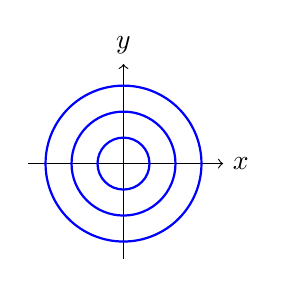
\begin{tikzpicture}[scale=0.55]
    \draw[->] (-2.2,0)--(2.3,0) node[right] {$x$};
    \draw[->] (0,-2.2)--(0,2.3) node[above] {$y$};
    \foreach \r in {0.6,1.2,1.8}{
        \draw[blue,thick] (0,0) circle (\r);
    }
\end{tikzpicture}

\small Circles
\end{minipage}
\hfill
\begin{minipage}[t]{0.31\linewidth}
\centering
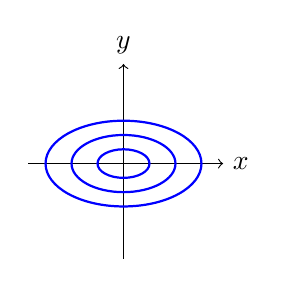
\begin{tikzpicture}[scale=0.55]
    \draw[->] (-2.2,0)--(2.3,0) node[right] {$x$};
    \draw[->] (0,-2.2)--(0,2.3) node[above] {$y$};
    \foreach \r in {0.6,1.2,1.8}{
        \draw[blue,thick]
            (0,0) ellipse [x radius=\r,y radius={0.55*\r}];
    }
\end{tikzpicture}

\small Axis-aligned ellipses
\end{minipage}
\hfill
\begin{minipage}[t]{0.31\linewidth}
\centering
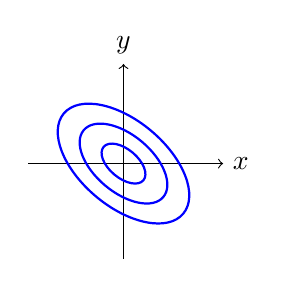
\begin{tikzpicture}[scale=0.55]
    \draw[->] (-2.2,0)--(2.3,0) node[right] {$x$};
    \draw[->] (0,-2.2)--(0,2.3) node[above] {$y$};
    \begin{scope}[rotate=-40]
        \foreach \r in {0.6,1.2,1.8}{
            \draw[blue,thick]
                (0,0) ellipse
                [x radius=\r,y radius={0.55*\r}];
        }
    \end{scope}
\end{tikzpicture}

\small Tilted ellipses
\end{minipage}
\caption{Possible shapes of trajectories around a center.}
\end{figure}

%-------------------------------------------------------------
\subsection{Determining the Direction}

The eigenvalues identify a center, but we still need
to determine whether trajectories move clockwise or
counterclockwise.

Choose a convenient point and evaluate
\[
\mathbf{x}'=A\mathbf{x}.
\]
This vector is tangent to the trajectory and points
in the direction of motion. At $(1,0)$, an upward
velocity indicates counterclockwise motion; a downward
velocity indicates clockwise motion.

\begin{example}[4]{
Classify the equilibrium and sketch the phase portrait:
\[
\mathbf{x}'=
\begin{pmatrix}
0&-2\\
2&0
\end{pmatrix}\mathbf{x}.
\]
}

\paragraph{Step 1. Find the eigenvalues.}
The characteristic equation is
\[
\lambda^2+4=0,
\]
so $\lambda=\pm2i$. Therefore, the origin is a center.

\paragraph{Step 2. Identify the trajectories.}
The system is
\[
x'=-2y,\qquad y'=2x.
\]
Notice that
\[
\frac{d}{dt}(x^2+y^2)
=2xx'+2yy'
=2x(-2y)+2y(2x)=0.
\]
Thus,
\[
x^2+y^2=C,
\]
so the trajectories are circles.

\paragraph{Step 3. Determine the direction.}
At $(1,0)$,
\[
\mathbf{x}'=
\begin{pmatrix}
0&-2\\
2&0
\end{pmatrix}
\begin{pmatrix}1\\0\end{pmatrix}
=
\begin{pmatrix}0\\2\end{pmatrix}.
\]
The velocity points upward. Hence, the origin is a
\[
\boxed{\text{counterclockwise center}.}
\]

\begin{center}
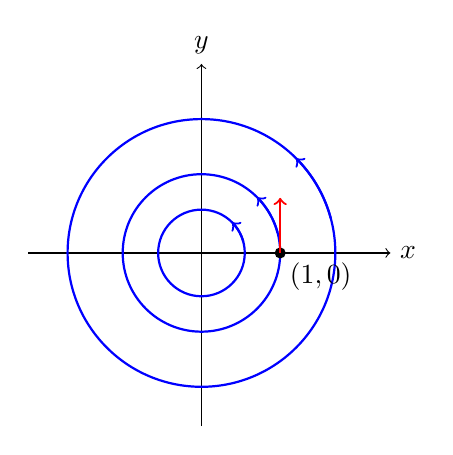
\begin{tikzpicture}[scale=1.0]
    \draw[->] (-2.2,0)--(2.4,0) node[right] {$x$};
    \draw[->] (0,-2.2)--(0,2.4) node[above] {$y$};

    \foreach \r in {0.55,1,1.7}{
        \draw[blue,thick] (0,0) circle (\r);
        \draw[blue,thick,->,domain=15:45,samples=20]
            plot ({\r*cos(\x)},{\r*sin(\x)});
    }

    \fill (1,0) circle (2pt);
    \node[below right] at (1,0) {$(1,0)$};
    \draw[red,thick,->] (1,0)--(1,0.7);
\end{tikzpicture}
\end{center}
The red arrow shows the velocity direction at $(1,0)$.
\end{example}

\begin{example}[5]{
Classify the equilibrium and determine the direction
of motion:
\[
\mathbf{x}'=
\begin{pmatrix}
3&2\\
-5&-3
\end{pmatrix}\mathbf{x}.
\]
}

\paragraph{Step 1. Find the eigenvalues.}
The characteristic equation is
\[
\begin{vmatrix}
\lambda-3&-2\\
5&\lambda+3
\end{vmatrix}
=\lambda^2+1=0.
\]
Thus, $\lambda=\pm i$, so the origin is a center.

\paragraph{Step 2. Determine the direction.}
At $(1,0)$,
\[
\mathbf{x}'=
\begin{pmatrix}
3&2\\
-5&-3
\end{pmatrix}
\begin{pmatrix}1\\0\end{pmatrix}
=
\begin{pmatrix}3\\-5\end{pmatrix}.
\]
The velocity points downward and to the right.
Therefore, the origin is a
\[
\boxed{\text{clockwise center}.}
\]
The trajectories are tilted ellipses, as shown below.

\begin{center}
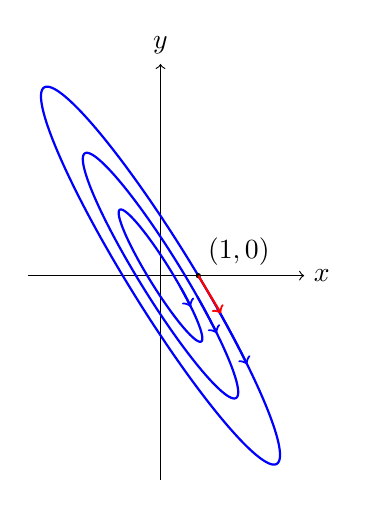
\begin{tikzpicture}[scale=0.48]
    \draw[->] (-3.5,0)--(3.8,0) node[right] {$x$};
    \draw[->] (0,-5.4)--(0,5.6) node[above] {$y$};

    % Exact trajectories through (r,0)
    \foreach \r in {0.35,0.65,1}{
        \draw[blue,thick,domain=0:360,samples=250]
            plot
            ({\r*(cos(\x)+3*sin(\x))},
             {-5*\r*sin(\x)});

        \draw[blue,thick,->,domain=10:28,samples=25]
            plot
            ({\r*(cos(\x)+3*sin(\x))},
             {-5*\r*sin(\x)});
    }

    \fill (1,0) circle (2pt);
    \node[above right] at (1,0) {$(1,0)$};
    \draw[red,thick,->] (1,0)--(1.6,-1);
\end{tikzpicture}
\end{center}
The red arrow is parallel to the velocity $(3,-5)$.
\end{example}

%%%%%%%%%%%%%%%%%%%%%%%%%%%%%%%%%%%%%%%%%%%%%%%%%%%%%%%%%%%%%%%%%%%%%%%%
\section{Spirals}

\subsection{The Effect of the Real Part}

For eigenvalues
\[
\lambda=\alpha\pm i\beta,
\qquad \alpha\ne0,\quad \beta\ne0,
\]
the solution contains oscillations multiplied by
$e^{\alpha t}$. The trajectories spiral around the origin.

\begin{itemize}
    \item If $\alpha<0$, the exponential factor decays.
    Trajectories spiral inward toward the origin.
    This is an \textbf{asymptotically stable spiral}.

    \item If $\alpha>0$, the exponential factor grows.
    Nonzero trajectories spiral outward.
    This is an \textbf{unstable spiral}.
\end{itemize}

Either type may rotate clockwise or counterclockwise.
As with centers, evaluate $A\mathbf{x}$ at a convenient
point to determine the direction.

%-------------------------------------------------------------
\subsection{Sketching a Spiral}

To sketch the phase portrait:
\begin{enumerate}
    \item Find the eigenvalues $\alpha\pm i\beta$.
    \item Use the sign of $\alpha$ to determine whether
    the motion is inward or outward.
    \item Evaluate $A\mathbf{x}$ at a convenient point
    to determine the direction of rotation.
    \item Draw representative spirals with arrows.
\end{enumerate}
The spirals need not be circular in shape. Their
precise shape depends on the matrix.

\begin{example}[6]{
Classify the equilibrium and sketch the phase portrait:
\[
\mathbf{x}'=
\begin{pmatrix}
-1&-4\\
1&-1
\end{pmatrix}\mathbf{x}.
\]
}

\paragraph{Step 1. Find the eigenvalues.}
The characteristic equation is
\[
\begin{vmatrix}
\lambda+1&4\\
-1&\lambda+1
\end{vmatrix}
=(\lambda+1)^2+4=0.
\]
Therefore,
\[
\lambda=-1\pm2i.
\]

\paragraph{Step 2. Determine stability.}
The real part is $\alpha=-1<0$, so trajectories
spiral inward. The origin is asymptotically stable.

\paragraph{Step 3. Determine the direction.}
At $(1,0)$,
\[
\mathbf{x}'=
\begin{pmatrix}
-1&-4\\
1&-1
\end{pmatrix}
\begin{pmatrix}1\\0\end{pmatrix}
=
\begin{pmatrix}-1\\1\end{pmatrix}.
\]
The velocity points upward and to the left.
Therefore, the origin is a
\[
\boxed{\text{counterclockwise stable spiral}.}
\]

\paragraph{Step 4. Sketch the trajectories.}
Draw counterclockwise spirals approaching the origin.

\begin{center}
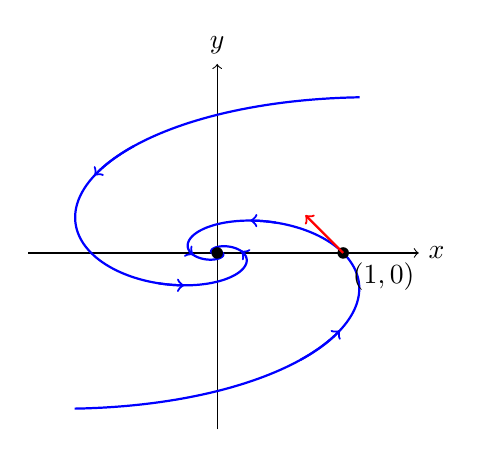
\begin{tikzpicture}[scale=1.6]
    \draw[->] (-1.5,0)--(1.6,0) node[right] {$x$};
    \draw[->] (0,-1.4)--(0,1.5) node[above] {$y$};

    % Exact trajectories, oriented as t increases
    \foreach \r in {-1,1}{
        \draw[blue,thick,domain=-1:5,samples=450]
            plot
            ({\r*exp(-\x)*cos(deg(2*\x))},
             {0.5*\r*exp(-\x)*sin(deg(2*\x))});

        \foreach \t in {-0.6,0.4,1.5}{
            \draw[blue,thick,->,
                  domain=\t:{\t+0.15},samples=20]
                plot
                ({\r*exp(-\x)*cos(deg(2*\x))},
                 {0.5*\r*exp(-\x)*sin(deg(2*\x))});
        }
    }

    \fill (0,0) circle (1.3pt);
    \fill (1,0) circle (1.3pt);
    \node[below right] at (1,0) {$(1,0)$};
    \draw[red,thick,->] (1,0)--(0.7,0.3);
\end{tikzpicture}
\end{center}
The red arrow shows the velocity direction at $(1,0)$.
\end{example}

\end{document}